\section{Parking lot problem}
\subsection{Part a)}
The MAPE and MASE of the model for the testing dataset is as follows:
\begin{itemize}[noitemsep]
	\item MAPE:  5.349685330136059
	\item MASE:  0.6598538430731961
\end{itemize}
\begin{figure}[h]
	\centering
	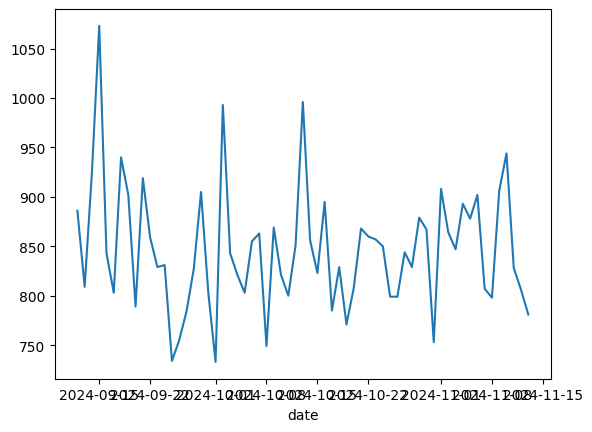
\includegraphics[width=0.5\textwidth]{1a_plot1.png}
	\caption{Number of cars entering each day}
\end{figure}

\begin{figure}[h]
	\centering
	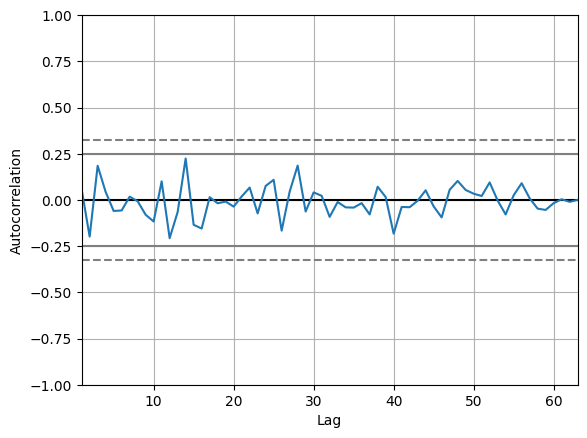
\includegraphics[width=0.5\textwidth]{1a_ac_plot.png}
	\caption{Auto correlation plot}
\end{figure}

\begin{figure}[h]
	\centering
	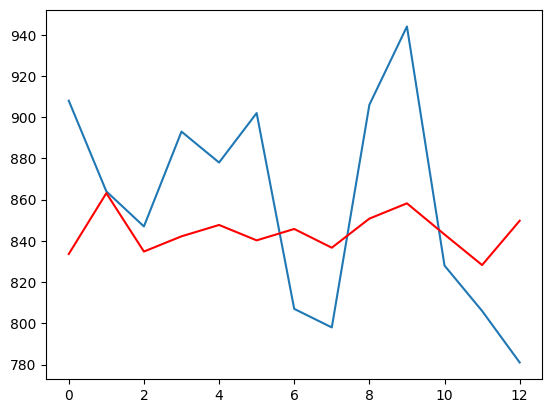
\includegraphics[width=0.5\textwidth]{1a_predictions.png}
	\caption{Predictions on test}
\end{figure}

\subsection{Part b)}
The MAPE and MASE of the model for the testing dataset is as follows:
\begin{itemize}[noitemsep]
	\item MAPE:  9.81429557710239
	\item MASE:  0.26311286911247267
\end{itemize}
\begin{figure}[h]
	\centering
	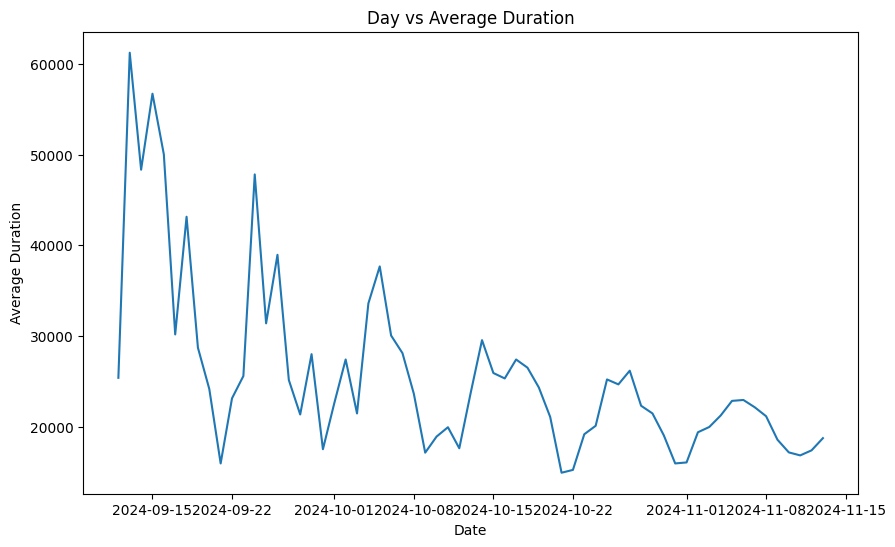
\includegraphics[width=0.5\textwidth]{1b_plot1.png}
	\caption{Number of cars entering each day}
\end{figure}

\begin{figure}[h]
	\centering
	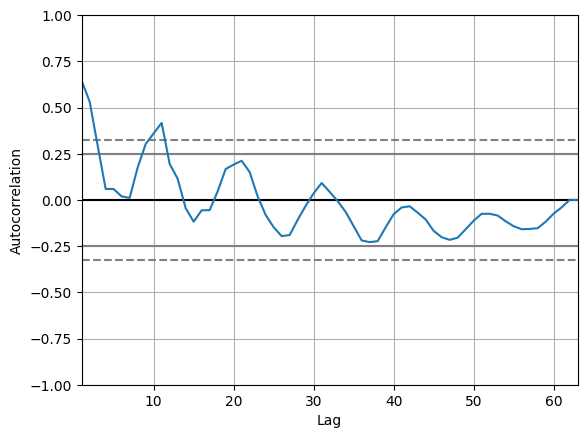
\includegraphics[width=0.5\textwidth]{1b_ac_plot.png}
	\caption{Auto correlation plot}
\end{figure}

\begin{figure}[h]
	\centering
	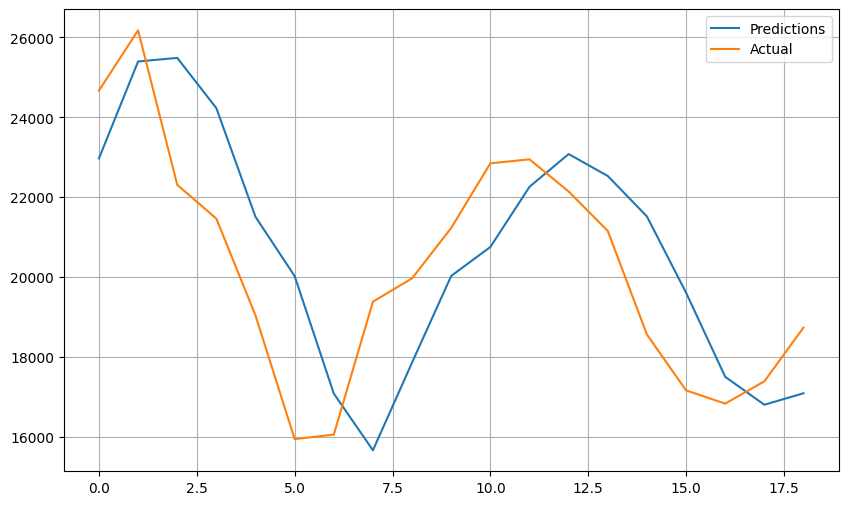
\includegraphics[width=0.5\textwidth]{1b_predictions.png}
	\caption{Predictions on test}
\end{figure}

\subsection{Part c)}
We have used the following smoothing techniques and the following results are achieved:
\begin{itemize}
	\item MAPE:  3.2338475891165857
	\item MASE:  0.17231581778569224
\end{itemize}

